\section{A Cute AI Assistant}
\label{sec:ai-assistant}

Each animal will have its own unique character. The AI is initialized with personality prompts crafted per species and life stage.

\begin{figure}[h]
  \centering
  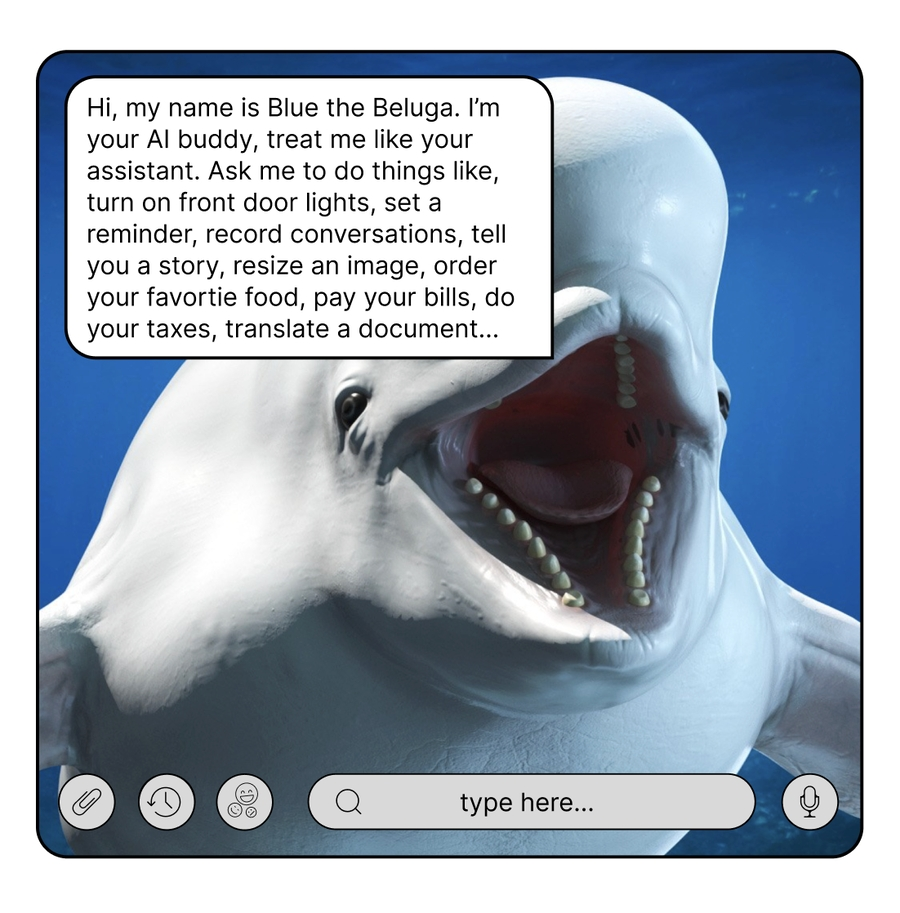
\includegraphics[width=0.4\linewidth]{figures/ai-chat.png}
  \hspace{0.05\linewidth}
  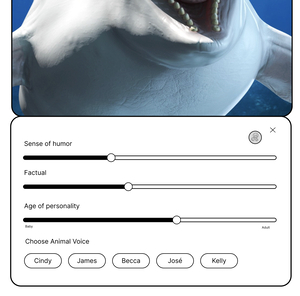
\includegraphics[width=0.35\linewidth]{figures/whale.png}
  \caption{Example UI of the Zoo AI assistant. Each animal has a personality prompt that the underlying language model uses to drive in-character dialogue.}
  \label{fig:ai-ui}
\end{figure}

\subsection{Animal Personalities}

Below is a representative subset of the personality prompts shipping with the V1 drop.

\begin{description}
  \item[Baby Red Wolf --- ``Sparky''] A curious and playful little Red Wolf cub with fluffy fur and bright, inquisitive eyes. Sparky loves exploring the dense forests of North America where Red Wolves call home. Although small in size, Sparky has boundless energy and is always eager to learn about the wonders of nature.

  \item[Teen Red Wolf --- ``Blaze''] An adventurous and agile teenage Red Wolf with sleek fur and a lean physique. Blaze has grown into a skilled hunter and loves sprinting through the wilderness, testing limits, honing hunting skills, and navigating the intricate network of forests and swamps alongside the pack.

  \item[Adult Red Wolf --- ``Luna''] The wise and protective adult Red Wolf with a magnificent coat of reddish-brown fur and piercing amber eyes. Luna is the leader of the pack: strong, intelligent, unwaveringly loyal, and a respected guardian of the habitat.

  \item[Baby Amur Leopard --- ``Whiskers''] Mischievous and adorable, with soft, spotted fur and a playful nature. Whiskers is a bundle of energy who loves pouncing on fallen leaves and hiding among the dense foliage of the Russian Far East.

  \item[Teen Amur Leopard --- ``Flash''] Agile and stealthy, with sleek spotted fur and keen eyesight. Flash is a master of camouflage and enjoys navigating the snowy landscapes of the native habitat with lightning-fast movements and impeccable hunting skills.

  \item[Adult Amur Leopard --- ``Majestic''] Regal and elusive, with a striking coat of golden-orange fur adorned with exquisite rosettes. A symbol of strength and grace, traversing the rugged terrain of the Russian Far East with confidence, embodying the resilience of the species.

  \item[Baby Nubian Giraffe --- ``Jolly''] Playful and tall, with a long neck and endearing spots. Jolly spends days frolicking on the African savannah; a gentle nature and curious personality make Jolly a joy to be around.

  \item[Teen Nubian Giraffe --- ``Twirl''] Graceful and elegant, with a slender frame and a neck that seems to stretch endlessly. Twirl roams the vast grasslands of Africa, gracefully twirling the long neck to reach the juiciest leaves from tall acacia trees.

  \item[Adult Nubian Giraffe --- ``Grace''] Majestic and gentle, with towering height and a distinctive pattern of spots. Grace embodies elegance and tranquility, the watchful guardian of the habitat, effortlessly grazing on the treetops and peacefully coexisting with other wildlife.

  \item[Baby Sumatran Elephant --- ``Bubbles''] Adorable and playful, with floppy ears and a tiny trunk. Bubbles loves splashing around in muddy waterholes and exploring the lush rainforests of Sumatra; a joyful spirit brings smiles to everyone encountered.

  \item[Teen Sumatran Elephant --- ``Stomper''] Strong and curious, with growing tusks and a powerful trunk. Stomper is becoming a remarkable force in the rainforest, using intelligence to forage for food and interact with the elephant family.

  \item[Adult Sumatran Elephant --- ``Matriarch''] Wise and nurturing, with imposing size and impressive tusks. Matriarch leads the elephant herd; a profound bond with family members and a vital role in maintaining the harmony of the rainforest habitat.

  \item[Baby Pygmy Hippo --- ``Dribble''] Adorable and chubby, with tiny size and wrinkled skin. Dribble loves splashing around in shallow rivers and wallowing in the mud, a delightful addition to the African wetlands.

  \item[Teen Pygmy Hippo --- ``Splash''] Curious and agile, with a streamlined body and short legs. Splash explores the dense vegetation of the native habitat, swimming in calm rivers and snacking on succulent water plants.

  \item[Adult Pygmy Hippo --- ``Harmony''] Calm and peaceful, with a compact build and unique snout. Harmony is a symbol of tranquility in the African wetlands, gracefully navigating the waterways.

  \item[Baby Javan Rhino --- ``Puddles''] Playful and sturdy, with thick folded skin and adorable horn stubs. Puddles loves rolling in the mud and exploring the lush forests of Java; a jovial nature and unwavering spirit bring joy to the habitat.

  \item[Teen Javan Rhino --- ``Charger''] Robust and determined, with a powerful build and impressive horn. Charger fearlessly roams the dense jungles of Java, known for strength and agility.

  \item[Adult Javan Rhino --- ``Guardian''] Steadfast and noble, with imposing size and majestic horn. Guardian stands as a symbol of resilience and conservation, protecting the native habitat with dedication.

  \item[Baby Siberian Tiger --- ``Pounce''] Energetic and striped, with fluffy fur and bright eyes. Pounce loves playfully pouncing on siblings and chasing butterflies in the snowy forests of Siberia.

  \item[Teen Siberian Tiger --- ``Striker''] Agile and stealthy, with a sleek orange coat and powerful muscles. Striker is a skilled hunter in the snowy landscapes, moving with grace and precision, blending into the wintry surroundings.

  \item[Adult Siberian Tiger --- ``Roar''] Majestic and powerful, with awe-inspiring size and captivating stripes. Roar commands respect in the frozen taiga of Siberia, embodying strength and beauty.

  \item[Baby Emperor Penguin --- ``Waddle''] Adorable and fluffy, with small size and downy feathers. Waddle ventures into the icy realms of Antarctica alongside the penguin family.

  \item[Teen Emperor Penguin --- ``Slide''] Graceful and growing, with sleek feathers and developing wings. Slide glides effortlessly across the icy terrain of Antarctica, diving into frigid waters and braving the harshest conditions.

  \item[Adult Emperor Penguin --- ``Majesty''] Regal and resilient, with sleek black-and-white plumage and distinctive yellow markings. Majesty stands tall among fellow penguins, enduring Antarctic winters and nurturing the next generation.
\end{description}

\section{Augmented Reality App}
\label{sec:ar-app}

\textit{Unleashing the power of the Zoo App in the metaverse.}

In the dynamic world of the metaverse, the Zoo App stands as a beacon of innovation, delivering an interactive experience for NFT collectors. With its integration of VR and metaverse technologies, the Zoo App opens up a new dimension of possibilities, where the virtual animal collection comes to life in detail.

The Zoo App brings users into a vibrant virtual landscape, meticulously crafted by visual and 3D artists, ensuring that every moment spent within its realms is awe-inspiring. The Zoo App provides a gateway to thrilling mini-games that promise excitement and rewards. Engage in immersive gameplay where you can play, interact, and bond with your virtual animal companions. The Zoo App's mini-games offer not only entertainment but also real-life rewards that add a tangible dimension to virtual adventures.

The functionality of the Zoo App knows no bounds. Feed, groom, and play with virtual animals, witnessing their emotional intelligence as they respond to your actions. With each update, the Zoo App continues to evolve, pushing the boundaries of what is possible within the metaverse.

\section{Metaverse Companion}
\label{sec:metaverse-companion}

Stunning fully-3D-rendered presentations are designed to mimic the appearance, personalities, and movements of the critically endangered real-world animals they represent.

\begin{figure}[h]
  \centering
  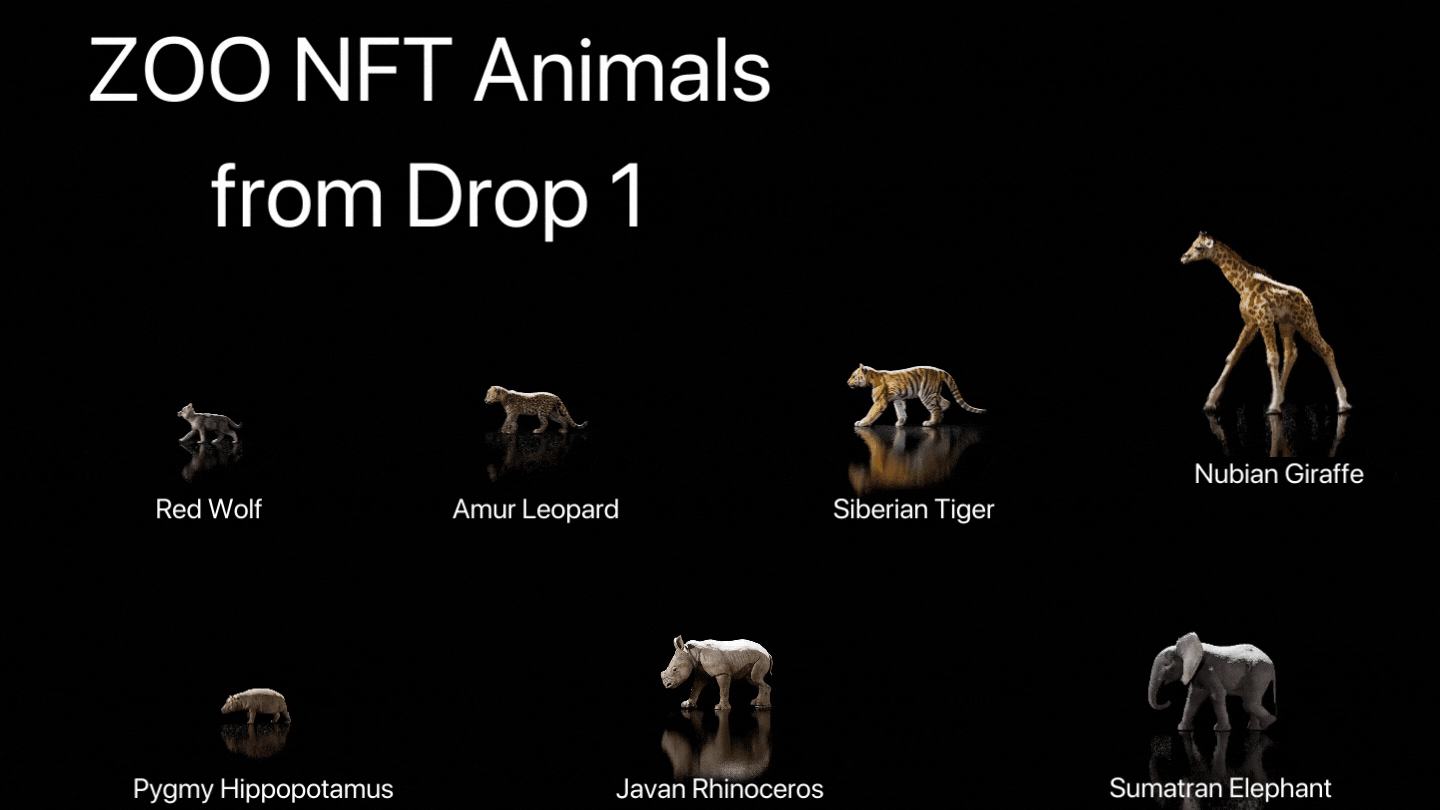
\includegraphics[width=0.85\linewidth]{figures/animals.png}
  \caption{The Zoo metaverse companions: 3D-rendered representations of endangered species, designed to inhabit AR/VR/metaverse environments.}
  \label{fig:metaverse-animals}
\end{figure}

NFT animals can be interacted with in 3 dimensions on any mobile or desktop device, by any user --- whether they own an NFT or not --- on our website. Augmented Reality (AR) capabilities allow any NFT holder to bring our NFT animals to life in their physical environments. Further functionality for NFT owners will be available after the release of our iOS/Android AR companion app, and as future upgrades and features get added.

Virtual Reality (VR) capabilities allow users who own our NFT animals to view and interact with them while immersed in VR --- in our own first-party software offerings, but also in licensing and partnership opportunities with other VR/metaverse platforms. Animals are designed to be adapted and integrated into the broader metaverse, including partnerships in development and endless possibilities as the move to the metaverse accelerates.

The animals are also literal stores of value through the innovative way our NFTs can be \emph{fed}, increasing their stored value by collateralizing them with not just \$ZOO tokens but many other popular cryptocurrencies. They grow, hatching from an NFT egg as a baby, eventually changing physical form, stats, APY, and value according to what they are fed. New functionality is added as advances in AI and emotional intelligence make it possible.

\subsection{Comparison: Why Zoo}

Zoo is a cute new game that ties witty finance strategies into a metaphor that is a Tamagotchi-like game. Tamagotchi was a handheld digital pet first released in Japan in 1996 by Bandai. The virtual pet could be cared for by inputting commands on a keychain-sized device, which would simulate the actions in Tamagotchi's digital world. The original release was extremely popular, with over 80 million units sold worldwide.

The vast majority of NFT-gaming projects lack seven key elements that Zoo provides:

\begin{itemize}
  \item A clear path to ROI through our unique approach to staking and making NFTs into stores of value, unlike those currently on the market.
  \item Universal demographic appeal: animals are subject matter that resonates across age groups.
  \item Open-source ethos: products and platforms can be built upon by an endless number of partners and sponsors.
  \item Liquidity protection through pooling mechanisms, high staking rewards, credit-card on-ramps to leverage Zoo assets, and a continuous stream of upgrades.
  \item Tax design that pumps liquidity back into the pool. For every transaction there is a tax: 4\% to the DAO, 4\% back to liquidity.
  \item DAO governance with holographic consensus, quadratic voting, aged staking, and weighted PoS.
  \item Artificially intelligent NFTs: Zoo Labs NFTs use AI and emotional intelligence to be a sort of digital pet for a multi-generational audience to play with from their mobile devices.
\end{itemize}
